\documentclass[french]{article}

%% Language and font encodings
\usepackage[utf8x]{inputenc}
\usepackage[T1]{fontenc}
\usepackage{babel}
\usepackage{float}
\usepackage{pdfpages}

%% Sets page size and margins
\usepackage[a4paper,top=3cm,bottom=2cm,left=3cm,right=3cm,marginparwidth=1.75cm]{geometry}

%% Useful packages
\usepackage{amsmath}
\usepackage{graphicx}
\usepackage[colorinlistoftodos]{todonotes}
\usepackage[colorlinks=true, allcolors=blue]{hyperref}

\newcommand\invisiblesection[1]{
\refstepcounter{section}
\addcontentsline{toc}{section}{\protect\numberline{\thesection}#1}
\sectionmark{#1}
}

\title{Sprint 1}
\author{Brandon Clement \& Kenji Fontaine \& Lucas Vivas}

\begin{document}
\maketitle

\section{Liste des taches}
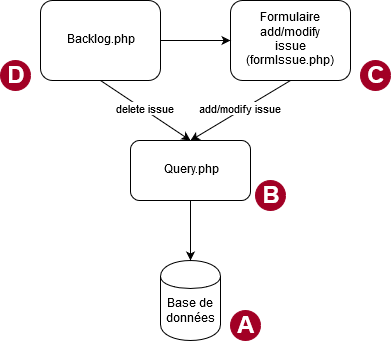
\includegraphics[scale=0.6]{rsc/archiSprint1.png}
\begin{itemize}
    \item $T_{Ad}$ (cout: 1/2 jh) : Design de la base de données permettant de stocker un backlog (plusieurs Issues).
    \item $T_{Ar}$ (cout: 1,5 jh) : Réalisation de la base de données permettant de stocker un backlog (plusieurs Issues).
    \item $T_{Bd}$ (cout: 1/2 jh) : Design de l'ensemble des requêtes permettant d'échanger avec la base de données (query.php).
    \item $T_{Br}$ (cout: 2 jh) : Réalisation de query.php.
    \item $T_{Cd}$ (cout: 1/2 jh) : Design du formulaire permettant d'ajouter une nouvelle issue (ID, Description, priorité, difficulté) à un backlog.
    \item $T_{Cr}$ (cout: 1,5 jh) : Réalisation du formulaire d'ajout d'une issue.
    \item $T_{Dd}$ (cout: 1/2 jh) : Design de la page permettant de visualiser la liste des issues existantes d'un backlog + modifier une issue + supprimer une issue.
    \item $T_{Dr}$ (cout: 2 jh) : Réaliser la page permettant de visualiser la liste des issues existantes + modifier une issue + supprimer une issue.

\end{itemize}

\section{Dépendances entre les taches}
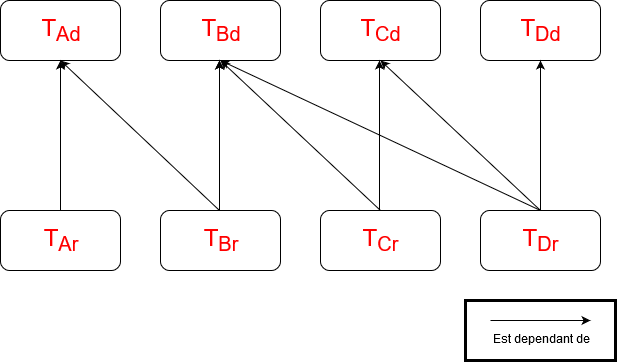
\includegraphics[scale=0.55]{rsc/task_dependancy_sprint_1.png}

\section{Taches pour les tests des US}
\begin{itemize}
    \item $T_{test1d}$ (cout: 1/2 jh, Issue 8) : Design du test : visualisation d'un backlog.
    \item $T_{test1r}$ (cout: 1/2 jh, Issue 8) : Réalisation du test : visualisation d'un backlog.
    \item $T_{test2d}$ (cout: 1/2 jh, Issue 10) : Design du test : modification d'une issue.
    \item $T_{test2r}$ (cout: 1/2 jh, Issue 10) : Réalisation du test : modification d'une issue.
    \item $T_{test3d}$ (cout: 1/2 jh, Issue 10) : Design du test : suppression d'une issue.
    \item $T_{test3r}$ (cout: 1/2 jh, Issue 10) : Réalisation du test : suppression d'une issue.
    \item $T_{test4d}$ (cout: 1/2 jh, Issue 9) : Design du test : ajouter une issue.
    \item $T_{test4r}$ (cout: 1/2 jh, Issue 9) : Réalisation du test : ajouter une issue.
\end{itemize}

\section{Diagramme de Pert}
\newpage
\rotatebox{90}{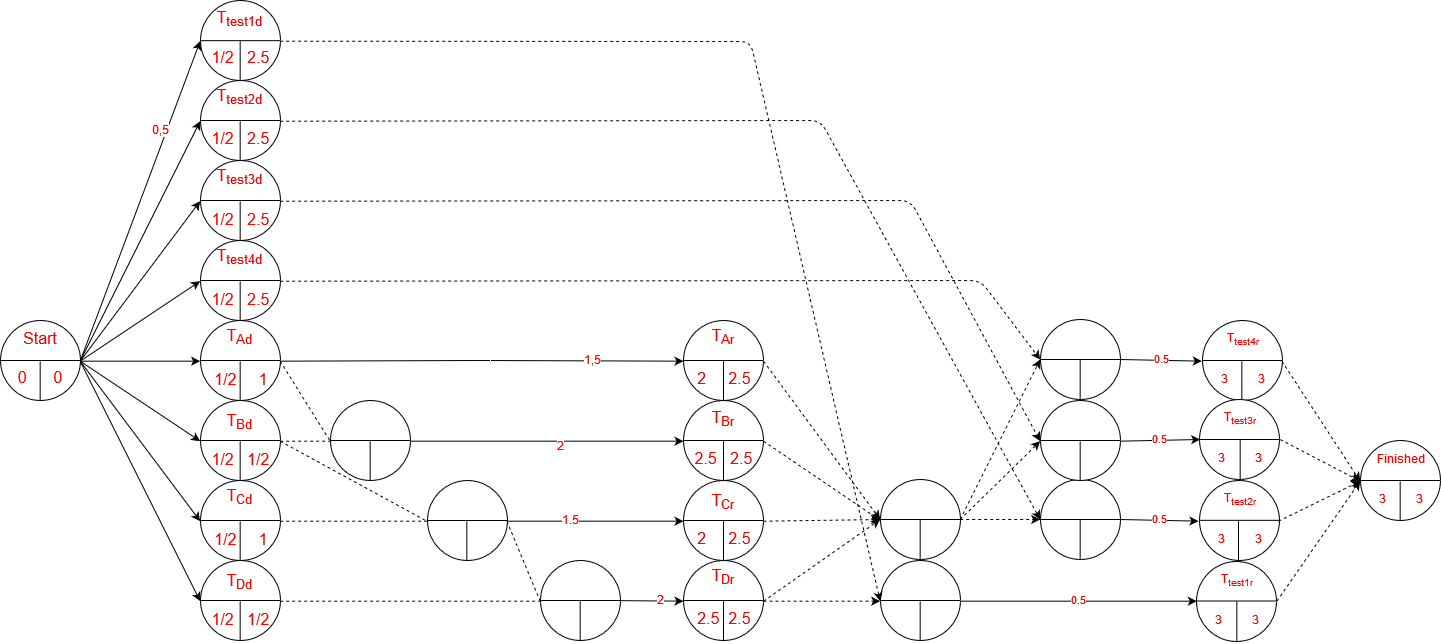
\includegraphics[scale=0.5]{rsc/sprint1_pertDiagram.png}}

\section{Planning}
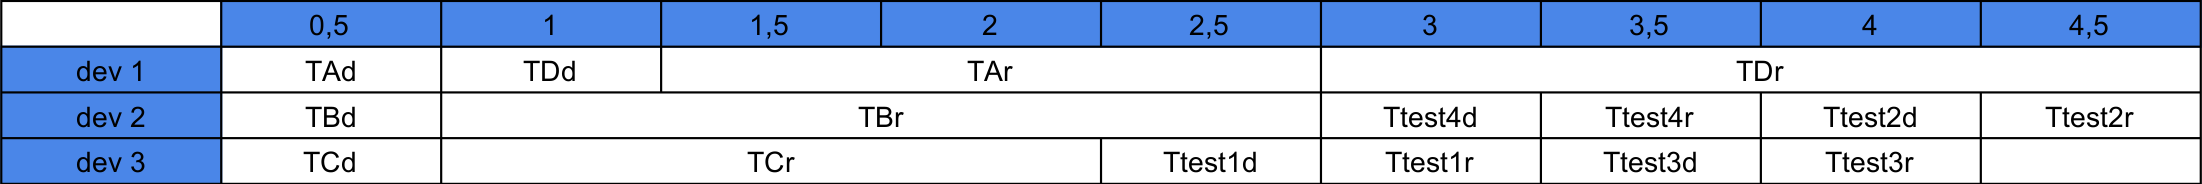
\includegraphics[scale=0.2]{rsc/planning_sprint1_nodate.png}

\section{Planning avec date}
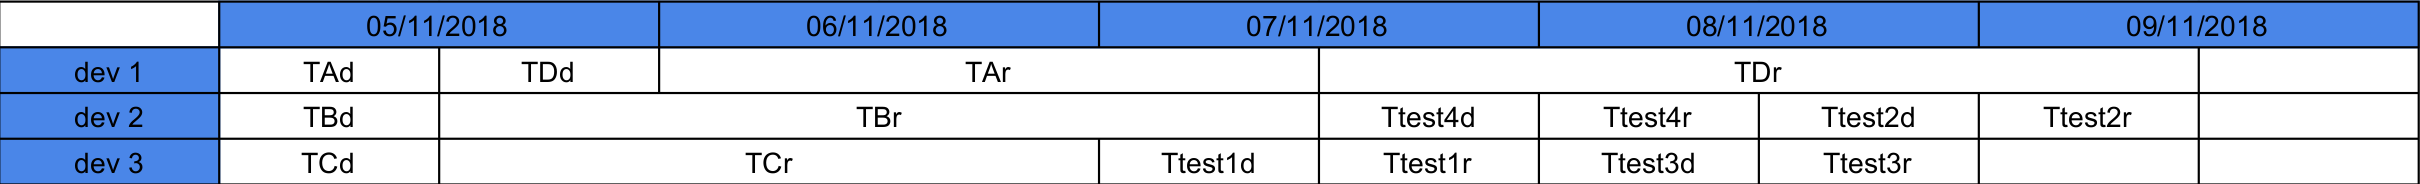
\includegraphics[scale=0.18]{rsc/planning_sprint1_date.png}

\end{document}
